\chapter{软件开发}
    \section{需求分析}
        \subsection{引言}
          \subsubsection{编写目的}
            本需求的编写目的在于研究无人机集群编队任务的开发途径和应用方法, 为以后的开发工作提供可靠的依据. 
          \subsubsection{项目背景}
            本课题的研究开发依赖于ROS平台, PX4开源飞控代码, QGC, 以及软件仿真平台(Gazebo), 硬件仿真平台(XPlane). 各自对应的关系如图\ref{simulator}所示. 
            \begin{figure}[htbp]
              \centering
              \subfigure[Software In the Loop]{
                  \begin{minipage}[t]{0.48\linewidth}
                  \centering
                  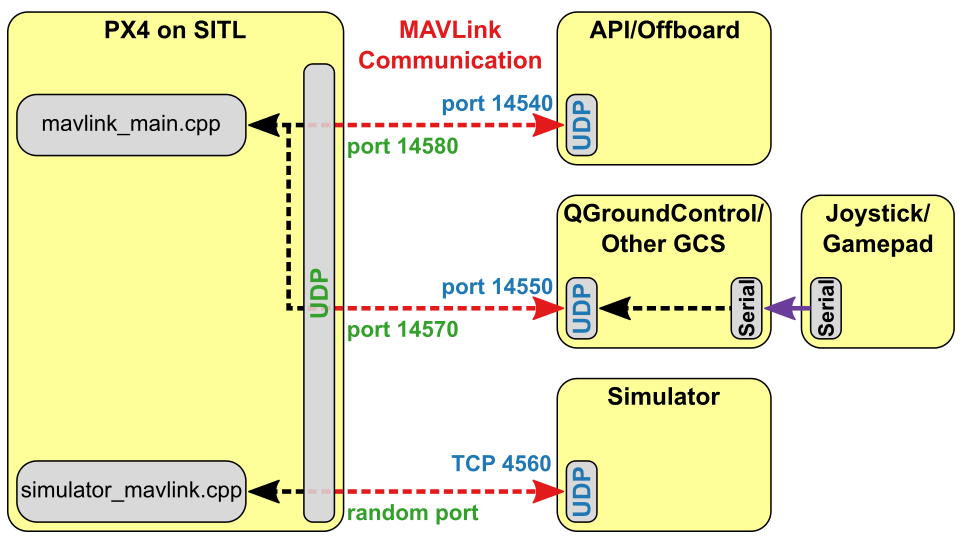
\includegraphics[width=0.9\textwidth]{pictures/sitl.png}
                  % \caption{Software In the Loop}
                  \end{minipage}%
              }%
              \subfigure[Software In the Loop]{
                \begin{minipage}[t]{0.48\linewidth}
                      \centering
                      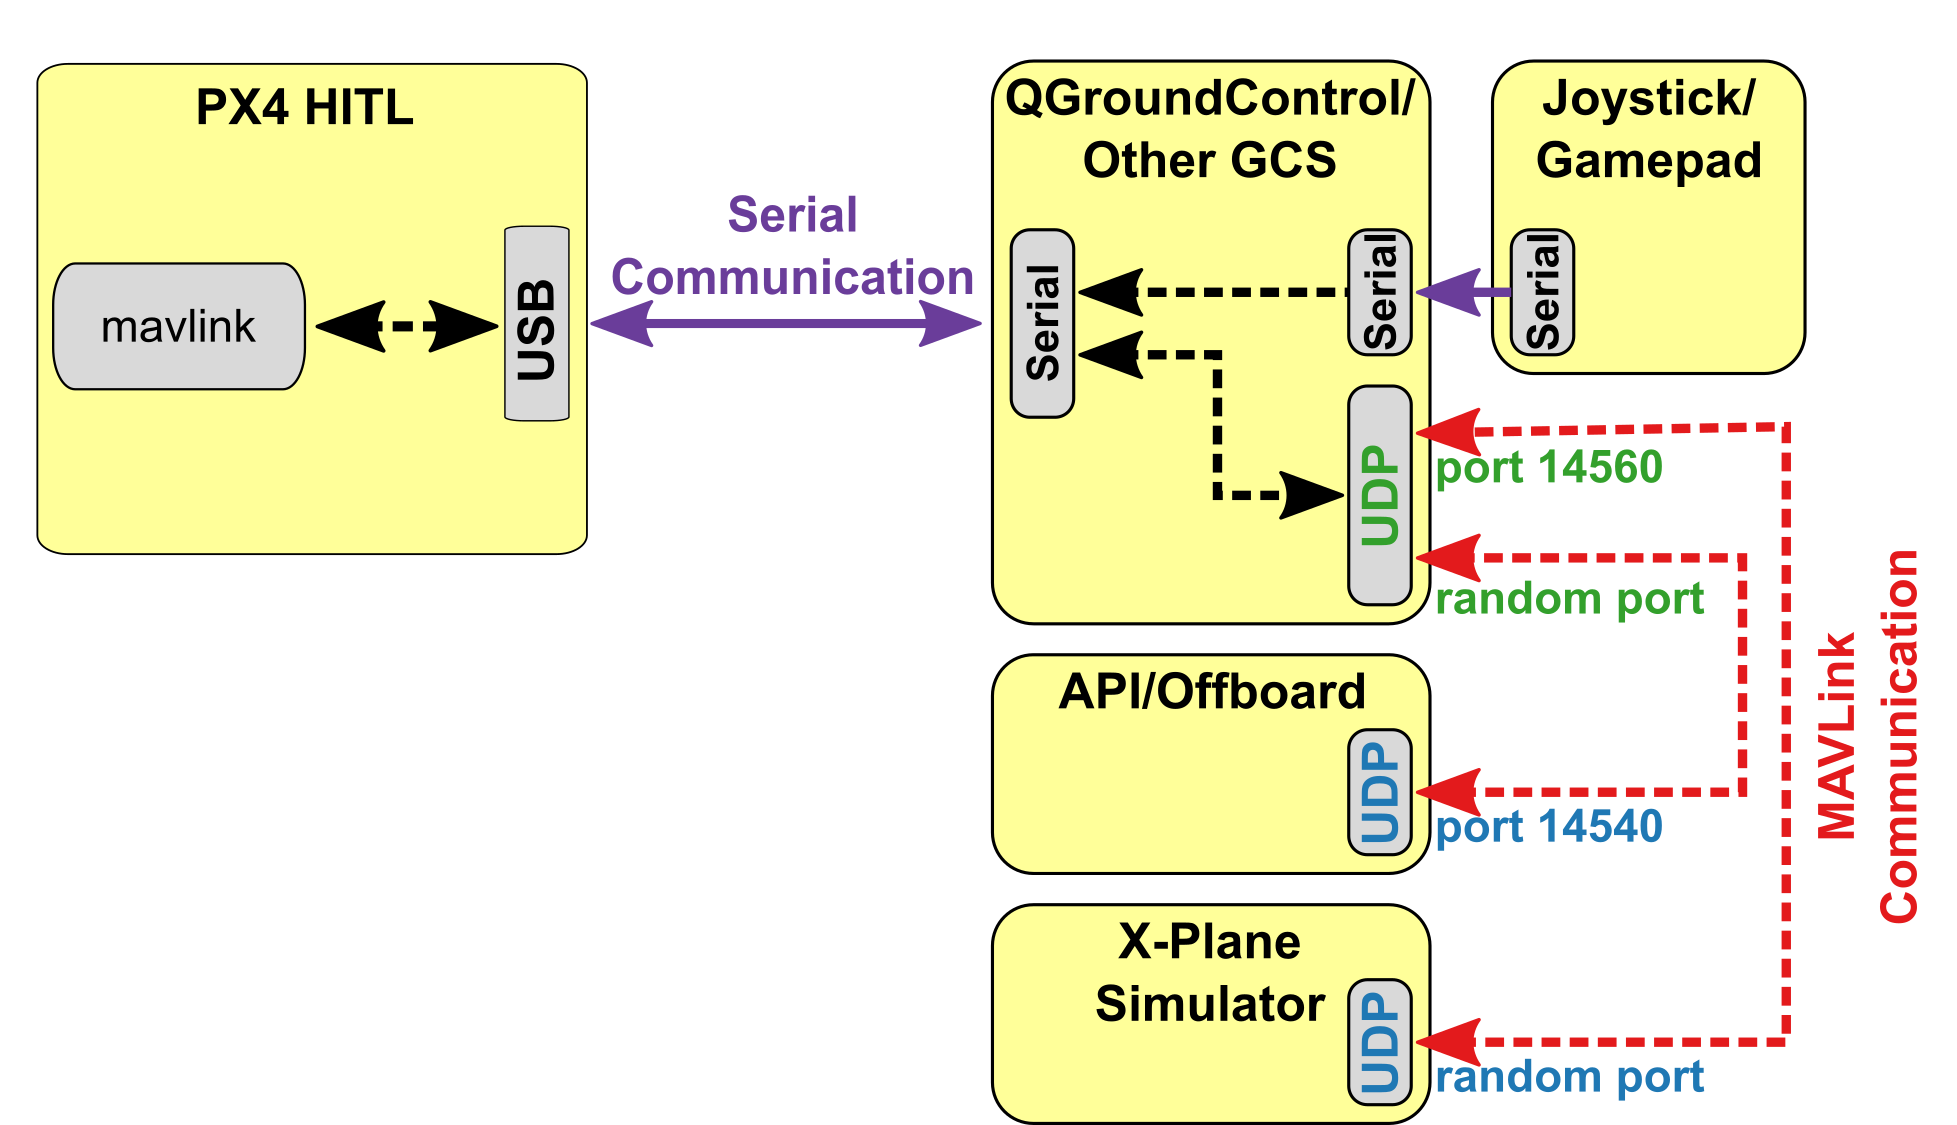
\includegraphics[width=0.9\textwidth]{pictures/hitl.png}
                      % \caption{Hardware In the Loop}
                  \end{minipage}%
              }%
              \caption{仿真平台}
              \label{simulator}
            \end{figure}
          
          \subsubsection{数据字典}
          \begin{itemize}
            \item [(1)] QGC$\_$COMMAND指令: 
            \item 用处: 集群地面站为每一架飞机发送的指令
            \item 组成: 飞机的id编号 + 飞机分组之后的组编号 + 主从机标志位 + 任务类型 + 其他的一些数据
          \end{itemize}
      
        \subsection{功能需求}
            把系统主要功能包括实时子系统, 导航子系统, 制导子系统, 姿态子系统, 通信子系统, 主控, 以及飞行日志记录. 
            其中实时子系统主要负责和PX4进行交互, 获取当前系统的实时位姿数据, 供其他子系统进行使用; 
            导航子系统包含了路径管理和期望航点的获取, 将其下发给制导子系统; 
            制导子系统包含了直线控制逻辑和盘旋控制逻辑, 并依托于控制逻辑计算期望姿态数据, 最后下发给姿态子系统; 
            姿态子系统负责将制导子系统获得的期望姿态进行PID控制,最终以某种方式将控制量发送给PX4;
            通信子系统在集群系统数据流下担任了主要角色, 它是无人机群组之间, 无人机相互之间, 无人机与集群地面站之间的沟通桥梁; 
            飞行日志记录主要担任着飞行数据的保存. 
            \par
            系统功能图如下: 
            \begin{figure}[htbp]
              \centering
              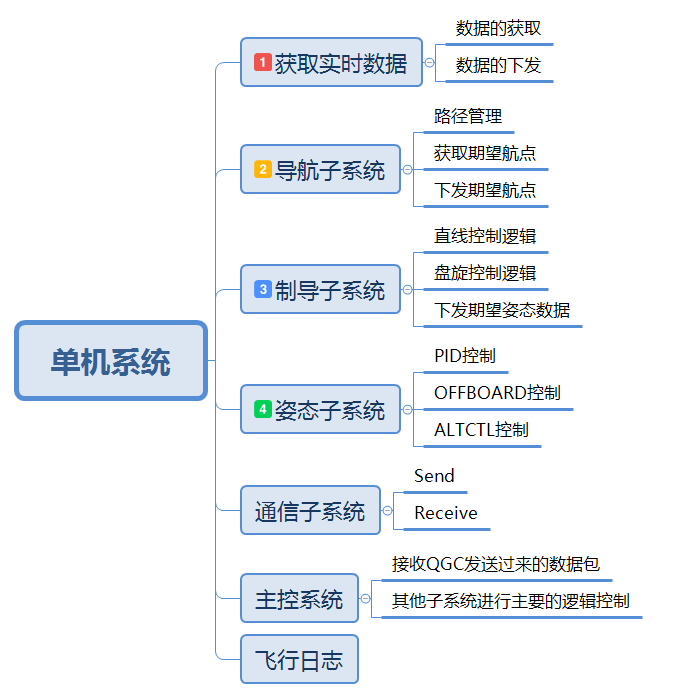
\includegraphics[width=0.5\textwidth]{pictures/single_system.png}
              \label{single_system}
            \end{figure}
    \clearpage
    \section{总体设计}
      \begin{figure}[h]
        \centering
        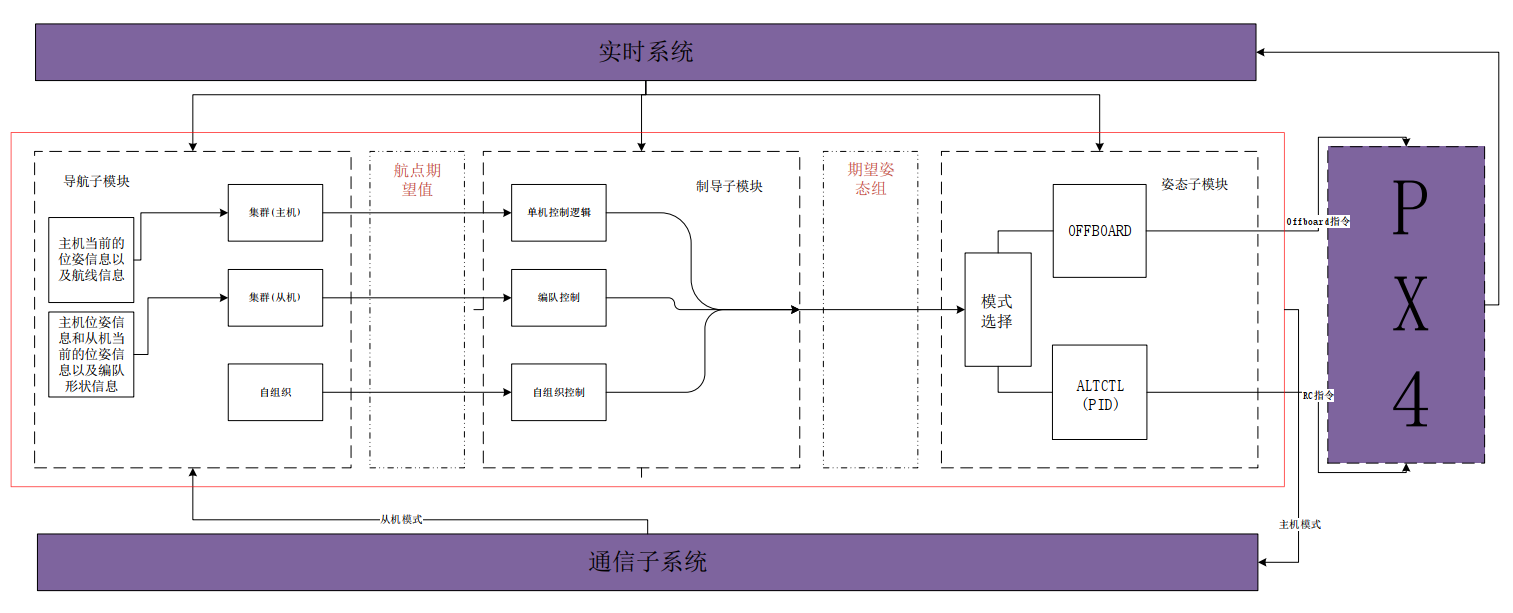
\includegraphics[width=\textwidth]{pictures/modules.png}
        \caption{UAV逻辑图}
        \label{fig:UAV}
      \end{figure}
        \subsection{处理流程}
        集群编队, 当所有飞机全部上电起飞后(\ref{fig:groups}), 等待集群地面站为每一架飞机发送指令(QGC$\_$COMMNAD), 对应无人机接收到集群地面站发送给自己的指令, 进行解析, 指定无人机当前的执行任务以及一个所属属性. \par
        若指定当前无人机为主机, 那么主机执行特定算法, 计算期望姿态组, 按照某种特定方式发布给PX4, 进而交给PX4的执行器进行执行, 同时广播自己特定的位姿数据到同组的无人机, 为后序的编队或者自组织服务, 数据流图见\ref{fig:leader}; 
        若指定当前无人机为从机, 那么接收其他无人机广播过来的位姿信息, 筛选出同组主机位姿信息, 进行计算, 完成特定任务, 见数据流图\ref{fig:follower}.
        
        \begin{figure}
          \centering
          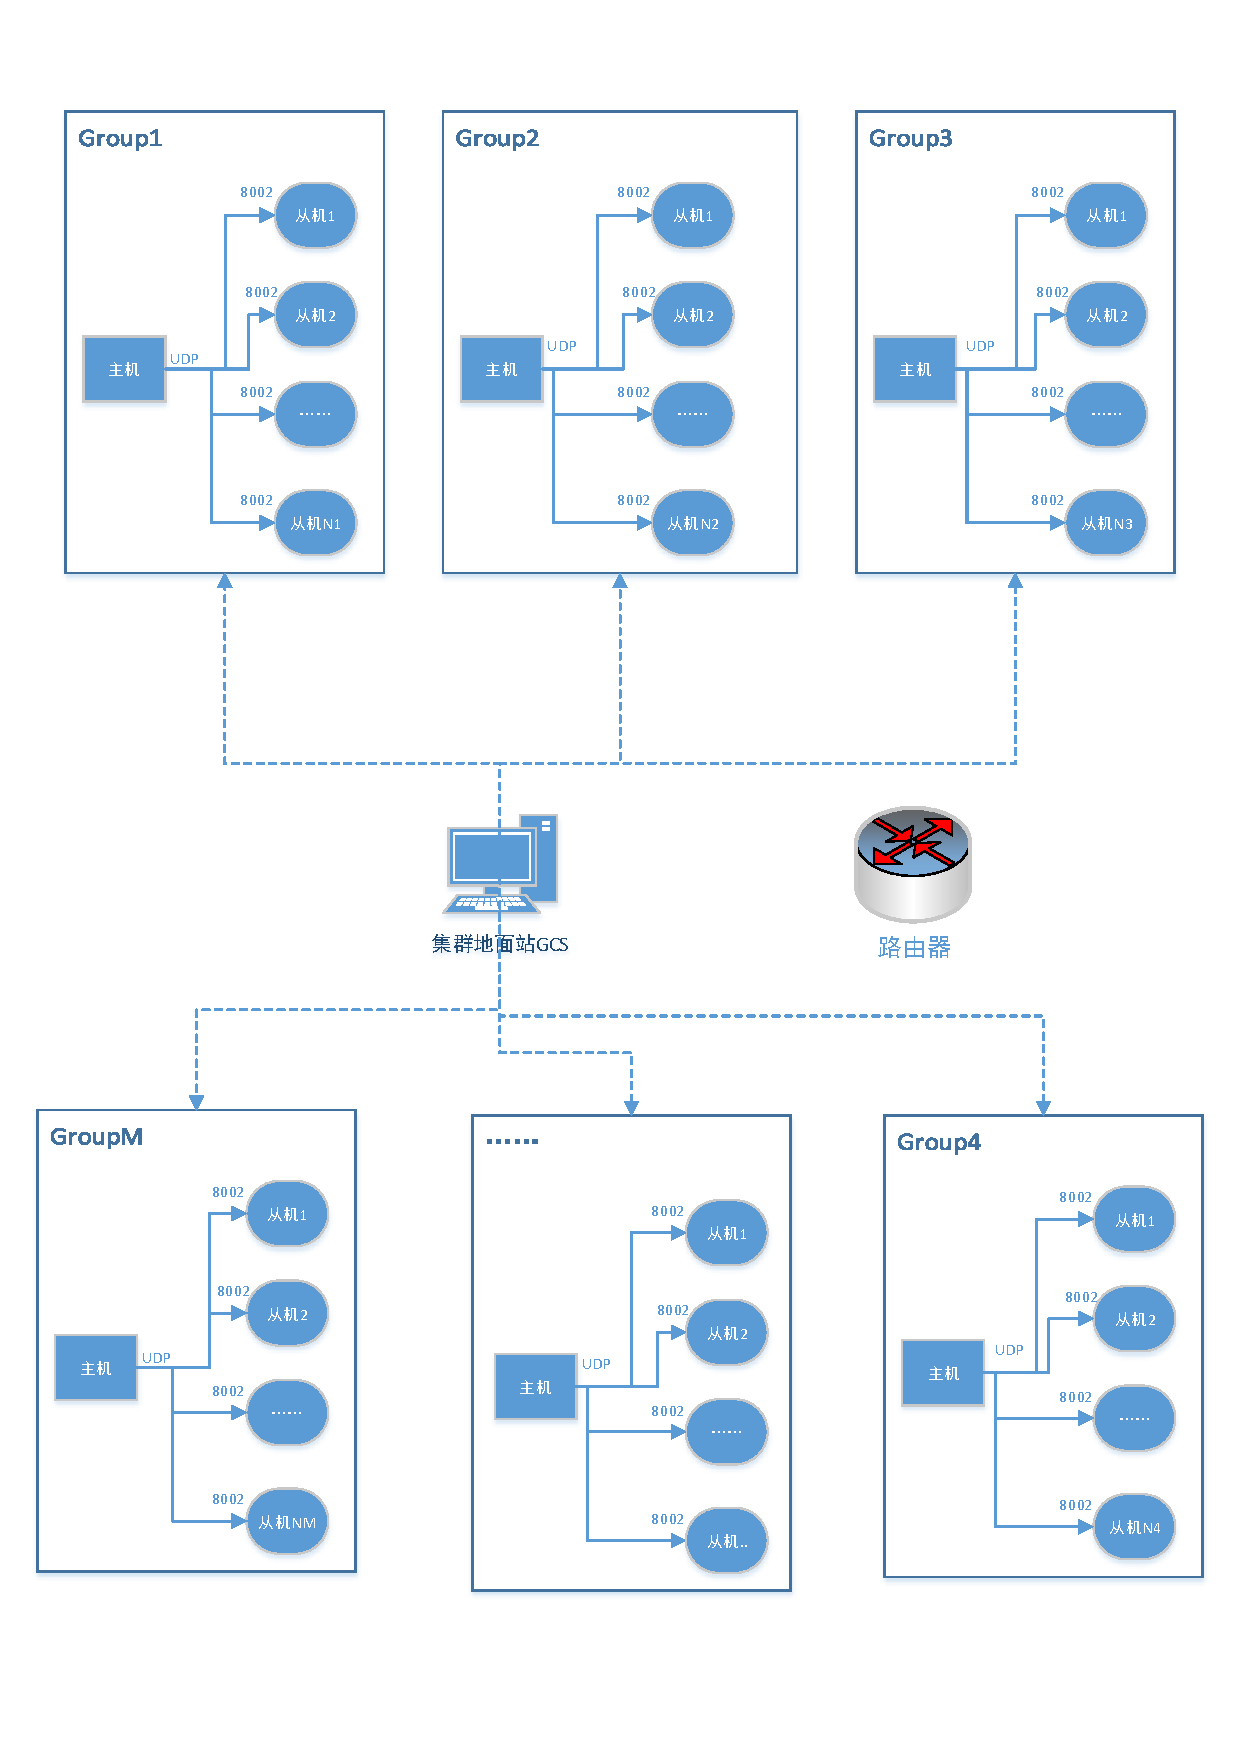
\includegraphics[width=\textwidth]{pictures/groups.pdf}
          \caption{组间分布图}
          \label{fig:groups}
        \end{figure}
        \begin{figure}
          \centering
          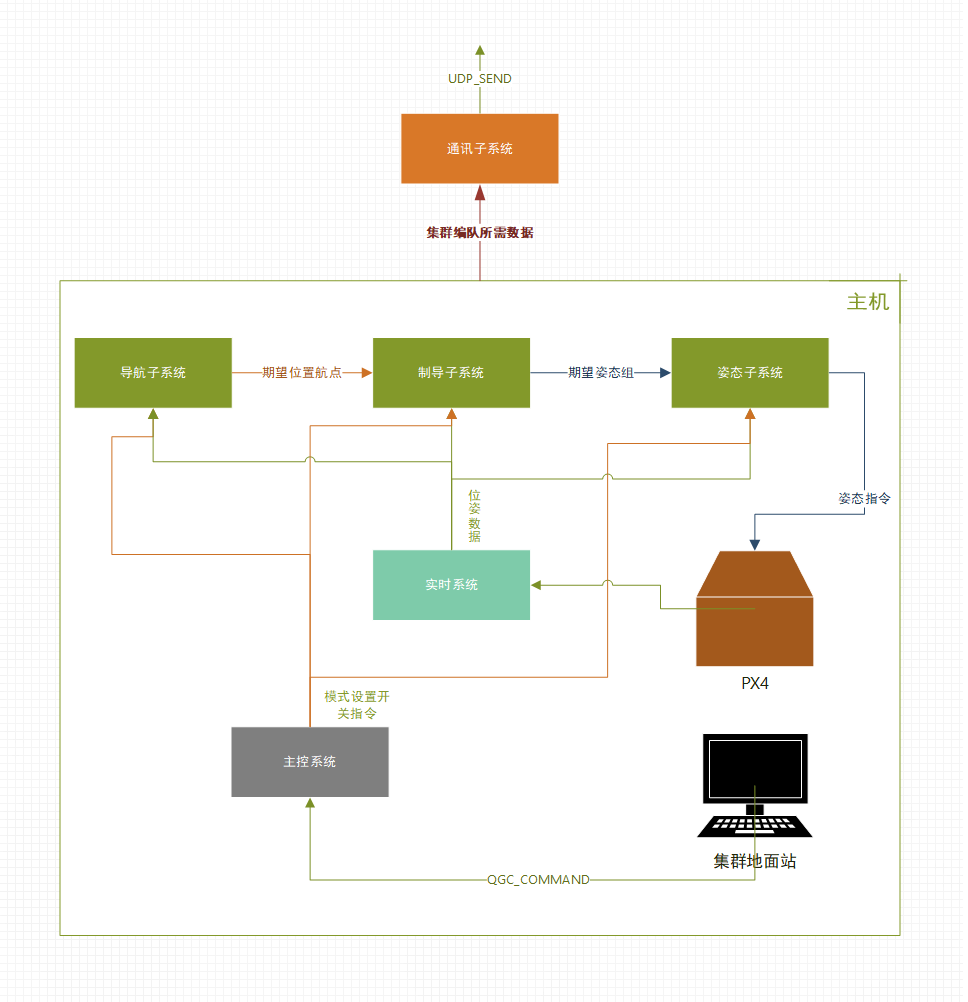
\includegraphics[width=\textwidth]{pictures/leader.png}
          \caption{主机数据流图}
          \label{fig:leader}
        \end{figure}
        \begin{figure}
          \centering
          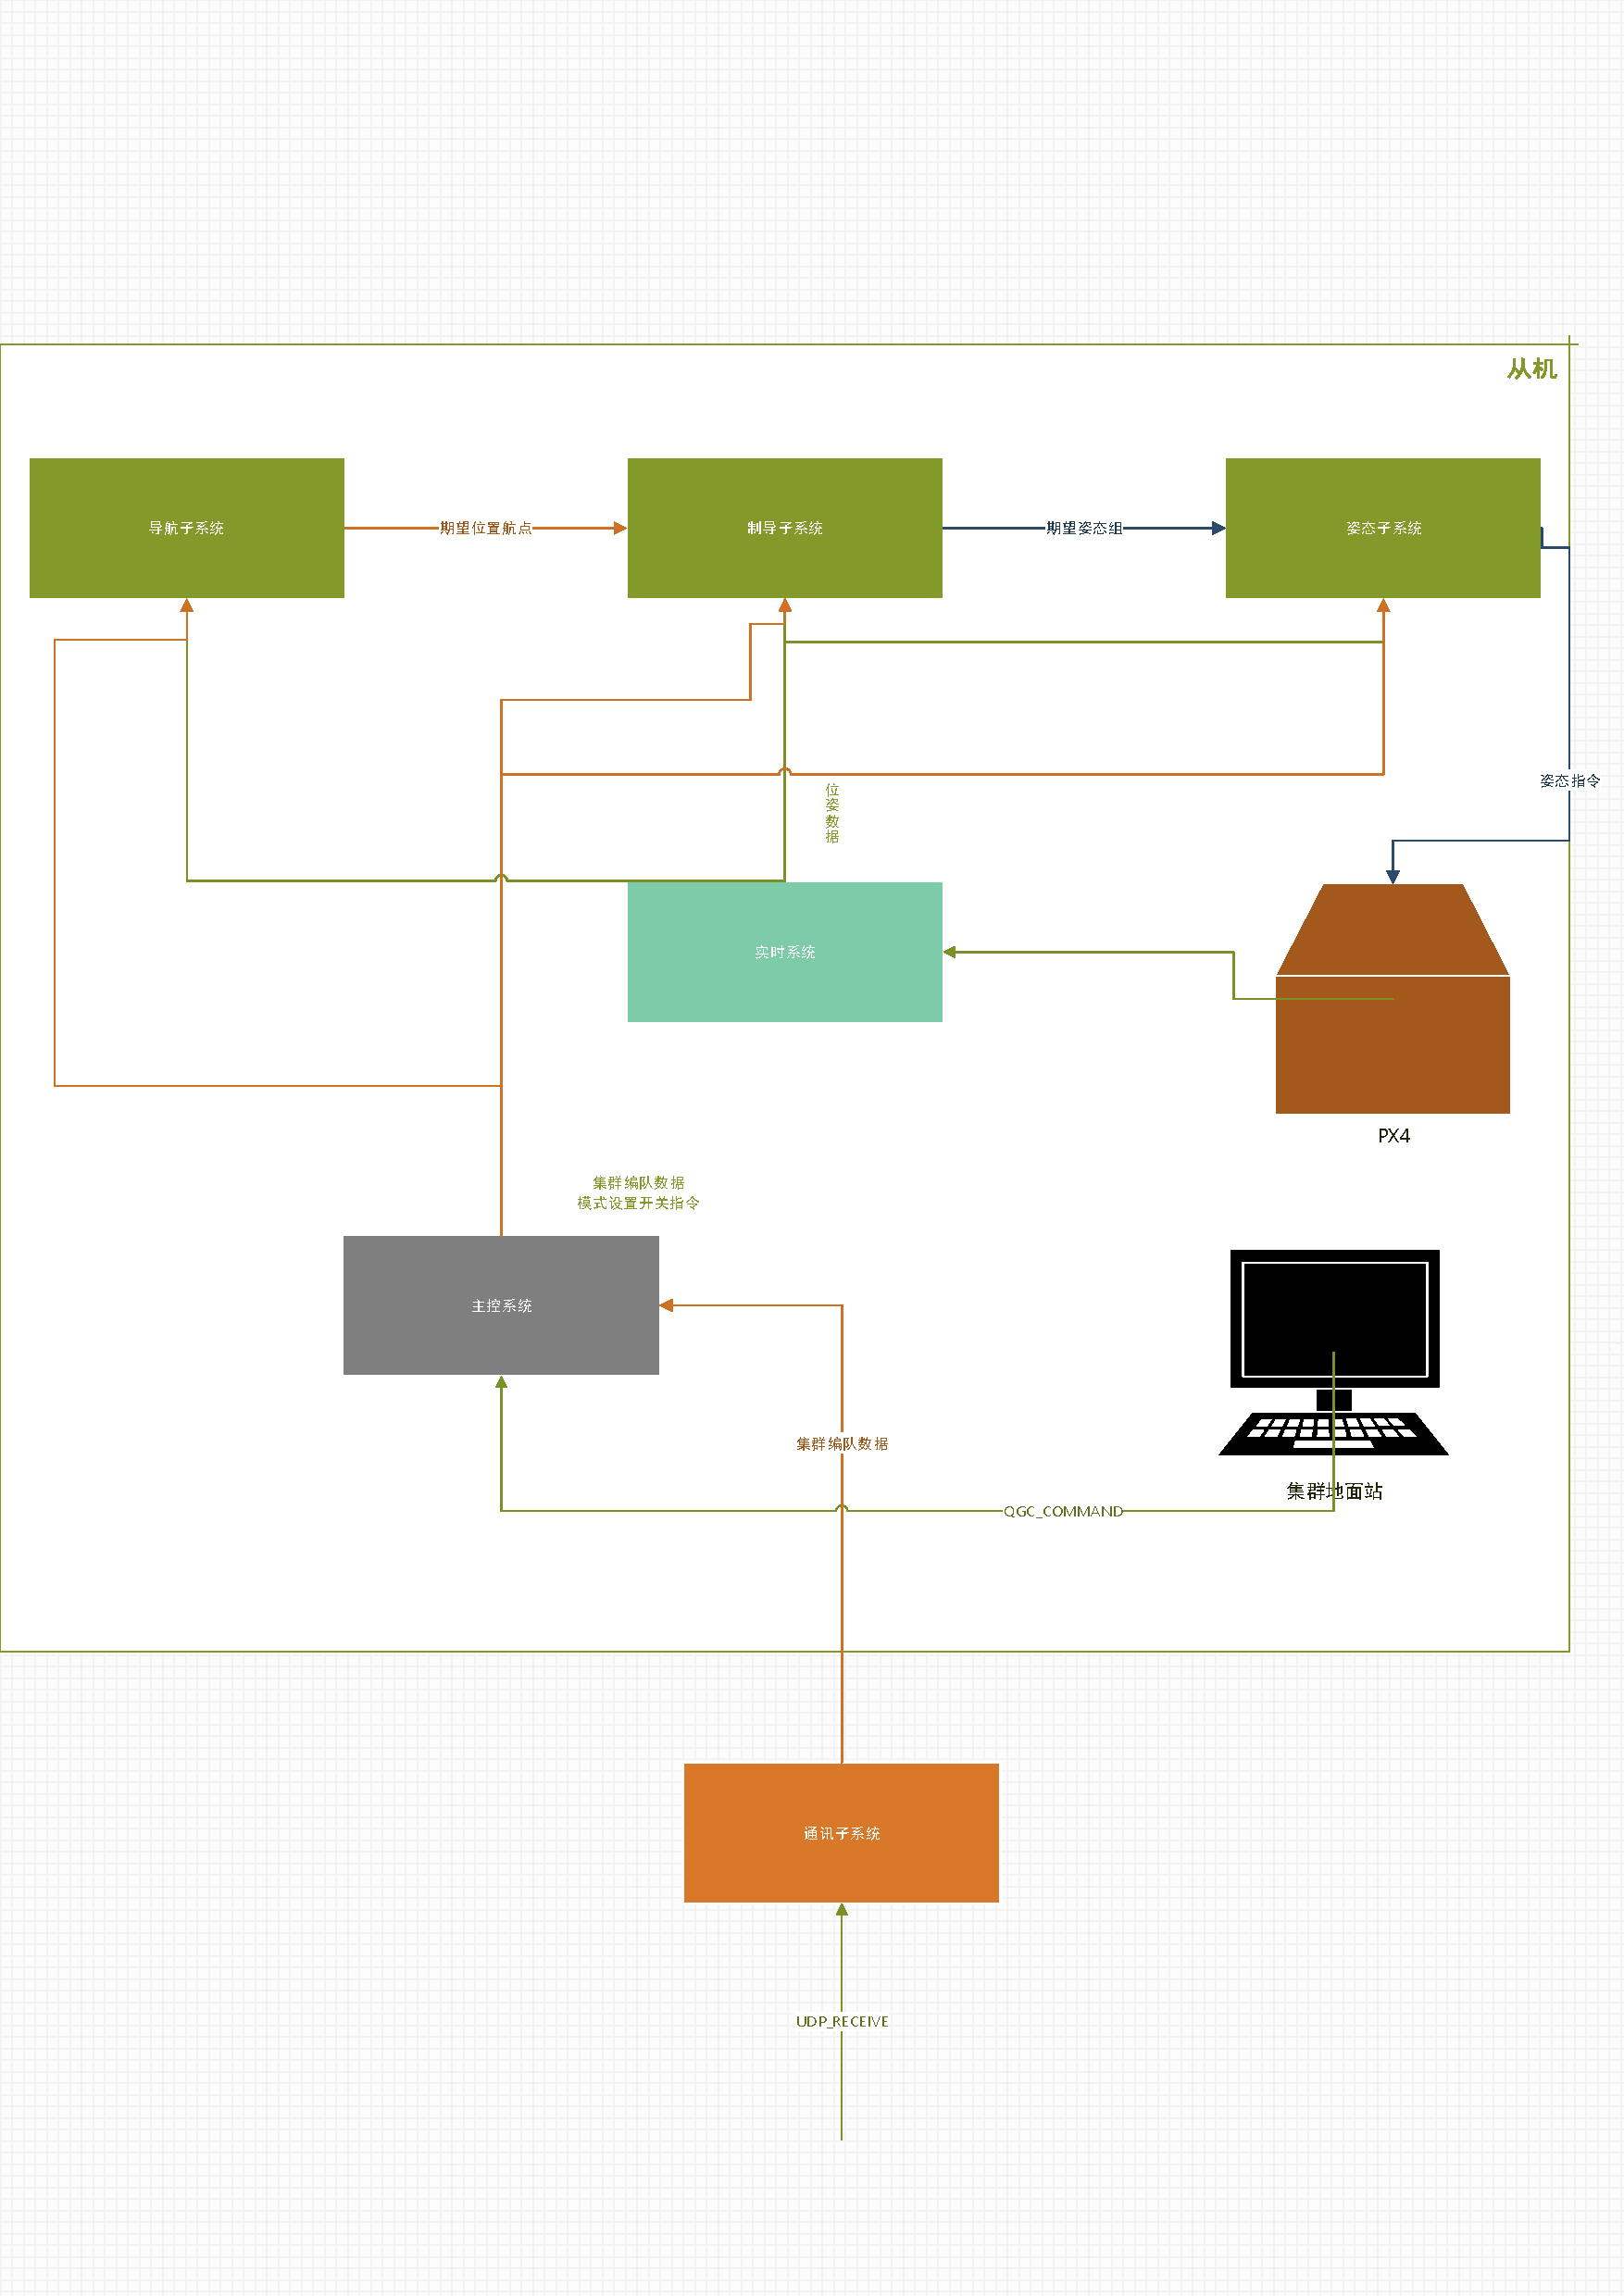
\includegraphics[width=\textwidth]{pictures/follower.pdf}
          \caption{从机数据流图}
          \label{fig:follower}
        \end{figure}

        \subsection{总体结构和模块外部设计}
        因每一架飞机根据任务分配的不同, 所属于的组名, 以及在组内所担任的角色也是变化的, 所以需要将主机和从机的两套执行控制逻辑整合成为一套, 在内部根据飞机控制模式进行判断选择所要执行的逻辑. 所以当前无人机的执行控制逻辑如图\ref{fig:UAV}所示. 
        
        
        \clearpage
    \section{详细设计}
      \subsection{无人机体系框架}
    本文探讨的主要内容包括固定翼姿态控制,飞行向导及自主导航等功能,
以层次化的观点来看,PX4由两个层次组成:一是飞行控制栈(flight stack),即自驾仪的软件解决方案,二是中间件,一种可以支持任意类型自主机器人的通用机器人中间件。
如图\ref{px4}所示。整个系统是反应式的。
箭头显示了模块之间最重要的连接的信息流。 实际上,连接比所示的多得多,并且大多数模块都可以访问一些特定的数据(例如,用于参数)。
模块通过使用名为uORB的发布-订阅消息总线相互通信,
使用“发布-订阅”方案意味着:系统是被动的,它是异步的,在有新数据可用时将立即更新
所有操作和通讯都完全并行化, 系统组件可以以线程安全的方式从任何地方使用数据.
其中,uORB(Micro Object Request Broker,微对象请求代理器)是PX4/Pixhawk系统中非常重要且关键的一个模块,它肩负了整个系统的数据传输任务,所有的传感器数据、GPS、PPM信号等都要从芯片获取后通过uORB进行传输到各个模块进行计算处理。实际上uORB是一套跨「进程」 的IPC通讯模块。在Pixhawk中,所有的功能被独立以进程模块为单位进行实现并工作。而进程间的数据交互就由为重要,必须要能够符合实时、有序的特点。

\begin{figure}
    \centering
    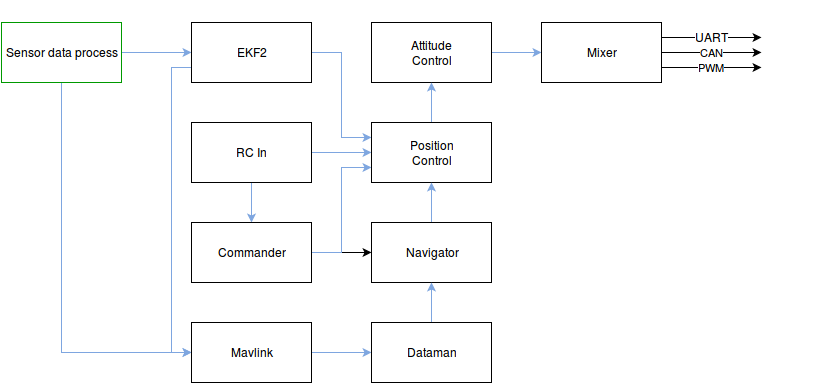
\includegraphics[width=0.5\textwidth]{pictures/PX4_Architecture_1.png}
    \caption{PX4}
    \label{px4}
\end{figure}
   
    其中, 飞行控制栈是用于自主无人机的制导,导航和控制算法的集合。 
    它包括用于固定翼,多旋翼和VTOL机身的控制器,以及用于姿态和位置的估计器。
图\ref{fight}显示了飞行堆栈的构建块的概述。它包含从传感器、RC输入和自动飞行控制(导航器)到电动机或伺服控制(执行器)的完整管道。
\begin{figure}[H]
    \centering
    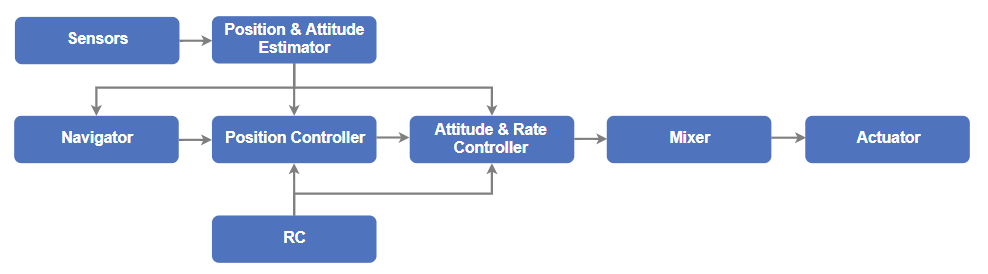
\includegraphics[width=0.6\textwidth]{pictures/fight_stack.png}
    \caption{fight stack}
    \label{fight}
\end{figure}
其中,estimator、controller 和 mixer 担当主要角色。
estimator 获取一个或多个传感器输入,对其进行组合,然后计算vehicle状态(例如,来自IMU传感器数据的姿态);
controller 是将设定值和测量或估计状态(过程变量)作为输入的组件,其目标是调整过程变量的值,使其与设定值匹配,输出是最终达到该设定点的校正。例如,位置控制器将位置设定值作为输入,过程变量是当前估计的位置,输出是将vehicle移向所需位置的姿态和推力设定点;
mixer 接受力指令(例如向右转)并将其转换为单独的电机指令,同时确保不超出某些限制,这种转换是特定于vehicle类型的,并且取决于各种因素,例如相对于重心的电动机布置或vehicle的旋转惯性。
本文主要对 controller 内部的算法进行了一定的改进。\par
控制器主要包括:导航控制器(navigator)、制导控制器(position controller)和姿态控制器(attitude controller)三层结构;同时,上层的输出也是下层的输入,之间紧密衔接,没有主次之分。
\subsection{导航控制器}
        导航就字面上说,就是引导航行的意思,而其确切的定义可表述为:导航是有目的地、
    安全有效地引导运动体(船只、潜艇、地面车辆以及飞机、宇宙飞船等). 也就是在当前位置已知的前提下,
    计算如何才能到达目的地,也即路径规划。本系统设计的导航子系统(navigator)执行流程如图\ref{fig:navigator}所示.
    \begin{figure}[htbp]
        \centering
        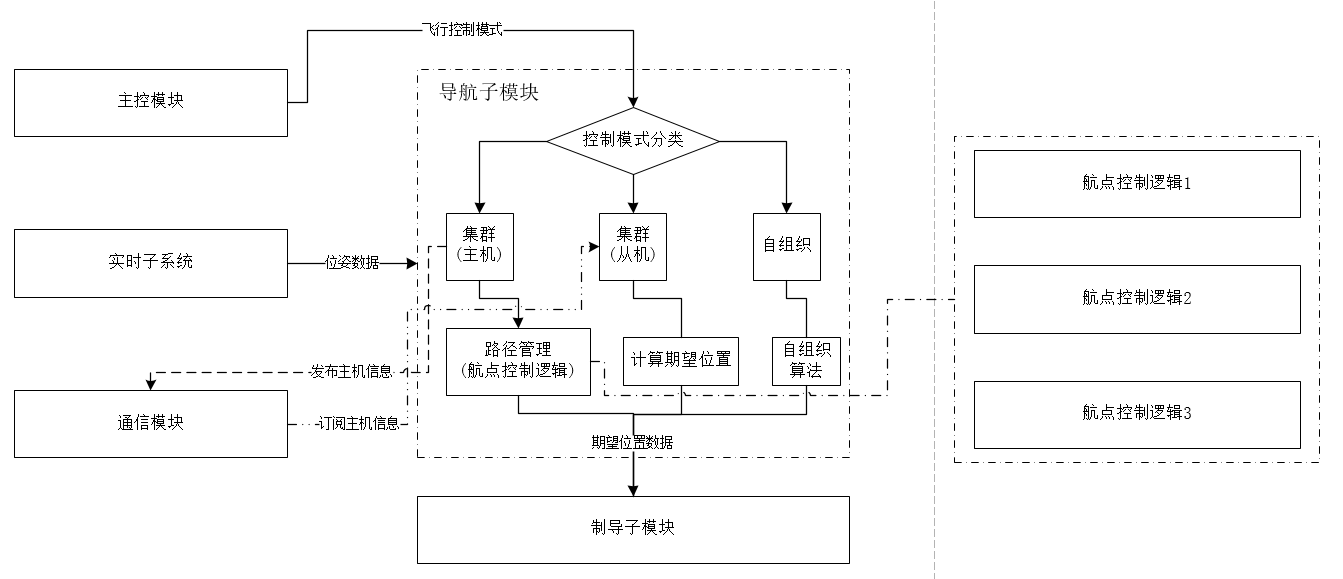
\includegraphics[width=\textwidth]{pictures/navigator.png}
        \caption{navigator}
        \label{fig:navigator}
    \end{figure}
    路径管理内部有三处控制逻辑, 分别对应着直线切换, 转弯圆角, 以及dubins曲线三种控制算法. 会在后面"算法"一节中进行介绍. 


\subsection{制导控制器}
    \chapter{position controller}

\section{Single vehicle}
    \subsection{offboard control logic}

    \clearpage
    \subsection{vf control logic}
    
    \clearpage

\section{Multiple vehicles}
    \subsection{fomation control logic}

    \clearpage

\section{Publishing date to attitude controller}
\subsection{姿态控制器}
    \chapter{attitude controller}

\section{offboard}


\subsection{mavros发送offboard数据流}
\begin{lstlisting}[title=publish messgae, frame=shadowbox]
    // 1. offboard publish (mavros topic)
    fixed_wing_local_att_sp_pub = nh.advertise<mavros_msgs::AttitudeTarget>("mavros/setpoint_raw/attitude", 10);
    
    #define MAVLINK_MSG_ID_SET_ATTITUDE_TARGET 82
      typedef struct __mavlink_set_attitude_target_t {
          uint32_t time_boot_ms; /*< [ms] Timestamp (time since system boot).*/
          float q[4]; /*<  Attitude quaternion (w, x, y, z order, zero-rotation is 1, 0, 0, 0)*/
          float body_roll_rate; /*< [rad/s] Body roll rate*/
          float body_pitch_rate; /*< [rad/s] Body pitch rate*/
          float body_yaw_rate; /*< [rad/s] Body yaw rate*/
          float thrust; /*<  Collective thrust, normalized to 0 .. 1 (-1 .. 1 for vehicles capable of reverse trust)*/
          uint8_t target_system; /*<  System ID*/
          uint8_t target_component; /*<  Component ID*/
          uint8_t type_mask; /*<  Mappings: If any of these bits are set, the corresponding input should be ignored: bit 1: body roll rate, bit 2: body pitch rate, bit 3: body yaw rate. bit 4-bit 6: reserved, bit 7: throttle, bit 8: attitude*/
     }) mavlink_set_attitude_target_t;
\end{lstlisting}
\section{Coordinated Turn 协调转弯}
\subsection{not being wind}
方向角的变化率是和机体的roll以及倾斜角(bank angle)有关系, 我们需要寻找一个简单的关系来帮助我们研究这种线性传递函数的关系 -- 协调转弯. \par
在协调转弯期间, 飞机在体坐标系下没有横向加速度. 从分析的角度来看, 协调转弯的一个假设运行我们得到一个简单的表达式将 heading rate 和 bank angle 联系起来. \par
协调转弯时, 为了无人机没有侧向力, bank angle $\phi$ 被设置.
在图\ref{fig:1}中, 作用在微型飞行器上的离心力与作用在水平方向上的升力的水平分量相等并相反。
\begin{figure}[htpb]
    \centering
    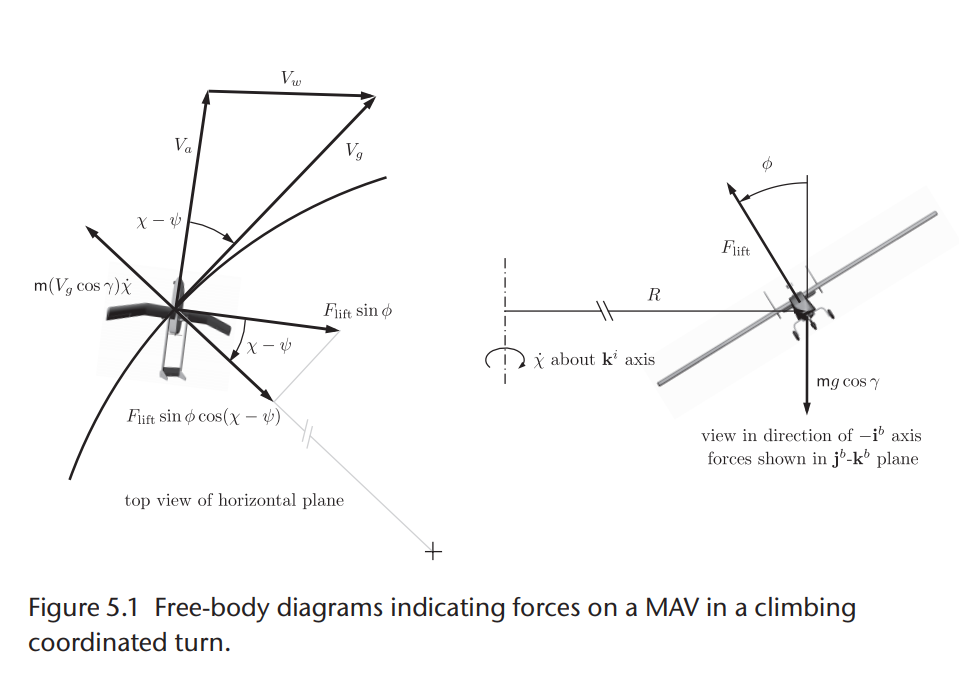
\includegraphics[width=0.8\textwidth]{pictures/5_1.png}
    \caption{爬升协调转弯MAV上的力}
    \label{fig:1}
\end{figure}
\par 作用在水平方向力的关系表示如下: 
\begin{align}
    F_{lift} sin \phi cos (\chi - \psi) &= m \frac{v^{2}}{R} \nonumber \\
    &= m v \omega \nonumber \\
    &= m (V_{g} cos \gamma) \dot{\chi} 
    \label{equ:1}
\end{align}
其中, $F_{lift}$代表的是升力, $\gamma$ 代表的是飞行轨迹的角度, $V_{g}, \chi$ 分别表示的是地速度以及方向角. \textcolor{red}{向心加速度的表达式: $a_{n} = \frac{v^{2}}{R} = v \omega$}
\par 离心力(The centrifugal force)(\textcolor{red}{$m (V_{g} cos \gamma) \dot{\chi} $})计算的时候, 用到了在惯性坐标系$k^{i}$上的方向角变化率$\dot{\chi}$ 和 速度的水平分量 $V_{a}cos \gamma$
\par 同样, 升力的垂直分量与重力在 $j^{b} - k^{b}$平面上的投影是等大反向的. 
垂直方向上的合力为:
\begin{equation}
    F_{lift} cos \phi = mg cos\gamma
    \label{equ:2}
\end{equation}
将等式\ref{equ:1}除以\ref{equ:2}得的 $\dot{\chi}$
\begin{equation}
    \dot{\chi} = \frac{g}{V_{g}} tan \phi cos(\chi - \psi)
    \label{equ:3}
\end{equation}
等式\ref{equ:3}就是协调转弯的表达式. 
\par 考虑到转弯半径等于 \textcolor{blue}{ $R = V_{g} \frac{cos \gamma}{\dot{\chi}}$}, 将上式代入半径中, 得到式子\ref{equ:4}. 在没有风或侧滑的情况下, 有\textcolor{red}{$V_{a} = V_{g}$和$\psi = \chi$}, 从而得到了式子\ref{equ:5}. 
\begin{equation}
    R = \frac{V_{g}^{2} cos \gamma}{g tan \phi cos(\chi - \psi)} 
    \label{equ:4}
\end{equation}
\begin{equation}
    \dot{\chi} = \frac{g}{V_{g}} tan \phi = \dot{\psi} = \frac{g}{V_{a}} tan \phi
    \label{equ:5}
\end{equation}
\par 在 9.2 节中, 我们将要介绍 在有风的情况下 \textcolor{blue}{$ \dot{\psi} = \frac{g}{V_{a}} tan \phi$} 该式子也成立
\clearpage
\subsection{being wind-Kinematic Model of Controlled Flight}
% 控制飞行动力学模型\par
在推导降阶表达式中, 简化的目的是估计运动中力平衡以及动量平衡的关系式(这些包含了 $\dot{u}, \dot{v}, \dot{\omega}, \dot{p}, , \dot{q}, \dot{r}$), 预估这些变量需要计算复杂的空气动力. 这些变量表达式可以被更简单的动力学表达式替代. 
这个更简单的动力学表达式是\textcolor{blue}{针对协调转弯和加速爬升的特定飞行条件而导出}.
\begin{figure}[htpb]
    \centering
    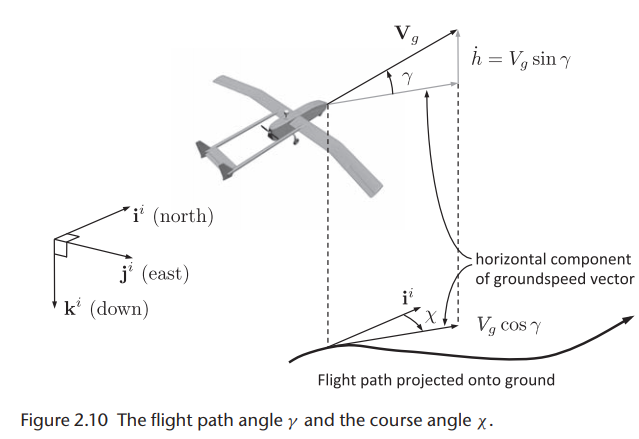
\includegraphics[width=0.8\textwidth]{pictures/2_10.png}
    \caption{航线轨迹角度$\gamma$和航向角$\chi$}
    \label{fig:2_10}
\end{figure}
针对图\ref{fig:2_10}, 飞机相对于惯性系的速度矢量可以用航向角和(惯性参考)飞行路径角表示为 
\begin{gather} % 输入多行公式
    V_{g}^{i} = V_{g} \begin{pmatrix}
        cos \chi cos \gamma \\
        sin \chi cos \gamma \\
        -sin \gamma \\
      \end{pmatrix}
      = \begin{pmatrix}
        \dot{p_{n}} \\
        \dot{p_{e}} \\
        \dot{h} \\
      \end{pmatrix}
      \label{equ:6}
  \end{gather}
\par 由于控制飞机的航向和空速是很常见的,因此用$\psi$和$V_{a}$表示等式\ref{equ:6}很有用. 
\begin{gather} % 输入多行公式
    V_{g} \begin{pmatrix}
        cos \chi cos \gamma \\
        sin \chi cos \gamma \\
        -sin \gamma \\
      \end{pmatrix} - \begin{pmatrix}
        w_{n} \\
        w_{e} \\
        w_{d} \\
      \end{pmatrix} =  V_{a} \begin{pmatrix}
        cos \psi cos \gamma_{a} \\
        sin \psi cos \gamma_{a} \\
        -sin \gamma_{a} \\
      \end{pmatrix}
      \label{equ:wind}
  \end{gather}
  结合风的表达式\ref{equ:wind}(地速等于空速加风速, 
    其中的 $\gamma_{a}$ 代表的是 空速的方向和水平方向的夹角), 我们可以得到
  \begin{gather} % 输入多行公式
    \begin{pmatrix}
        \dot{p_{n}} \\
        \dot{p_{e}} \\
        \dot{h} \\
      \end{pmatrix} = V_{a} \begin{pmatrix}
        cos \psi cos \gamma_{a} \\
        sin \psi cos \gamma_{a} \\
        sin \gamma_{a} \\
      \end{pmatrix} +  \begin{pmatrix}
        w_{n} \\
        w_{e} \\
        -w_{d} \\
      \end{pmatrix}
      \label{equ:7}
  \end{gather}
  如果我们假设飞机保持在一个恒定的高度,并且没有向下的风分量,那么运动学表达式简化为\ref{equ:8}, 同样该模型也是无人机领域中比较常用的模型. 
  \begin{gather} % 输入多行公式
    \begin{pmatrix}
        \dot{p_{n}} \\
        \dot{p_{e}} \\
        \dot{h} \\
      \end{pmatrix} = V_{a} \begin{pmatrix}
        cos \psi \\
        sin \psi \\
        0 \\
      \end{pmatrix} +  \begin{pmatrix}
        w_{n} \\
        w_{e} \\
        0 \\
      \end{pmatrix}
      \label{equ:8}
  \end{gather}
  \subsection{Coordinated Turn}
  之前的协调转弯的表达式为 $\dot{\chi} = \frac{g}{V_{g}} tan \phi cos(\chi - \psi)$. 
  即使在第6章中描述的自动驾驶回路并没有强制执行协调转弯条件,
  飞机必须倾斜才能转弯(而不是打滑才能转弯)这个基本条件已经被这个模型捕捉到了。\par
  协调转弯可以被 heading 和 空速进行表示. 我们先对\ref{equ:wind}两边进行求导, 得到下面的式子\ref{equ:9}
  \begin{gather} % 输入多行公式
    \begin{pmatrix}
        cos \chi cos \gamma & - V_{g} sin \chi cos \gamma & - V_{g} cos \chi sin \gamma \\
        sin \chi cos \gamma & V_{g} cos \chi cos \gamma & - V_{g} sin \chi sin \gamma \\
        -sin \gamma & 0 & -cos \gamma \\
      \end{pmatrix} \begin{pmatrix}
        \dot{V_{g}} \\
        \dot{\chi} \\
        \dot{\gamma} \\
    \end{pmatrix}
      = \begin{pmatrix}
        cos \psi cos \gamma_{a} & - V_{a} sin \psi cos \gamma_{a} & - V_{a} cos \psi sin \gamma_{a} \\
        sin \psi cos \gamma_{a} & V_{a} cos \psi cos \gamma_{a} & - V_{a} sin \psi sin \gamma_{a} \\
        -sin \gamma_{a} & 0 & -cos \gamma_{a} \\
      \end{pmatrix} \begin{pmatrix}
        \dot{V_{a}} \\
        \dot{\psi} \\
        \dot{\gamma_{a}} \\
    \end{pmatrix}
      \label{equ:9}
  \end{gather}
  \par 在定高和没有向下风分量的情况下, $\gamma, \gamma_{a}, \dot{\gamma}, \dot{\gamma_a}$ 和 $w_{d}$ 都是0, 根据$\dot{V_{a}}$ 和$\dot{\chi}$求解$\dot{V_{g}}$ 和$\dot{\psi}$
  \begin{equation}
    \begin{split}
      \dot{V_{g}} &= \frac{\dot{V_{a}}}{cos (\chi - \psi)} + V_{g} \dot{\chi} tan(\chi - \psi) \\
      \dot{\psi} &= \frac{\dot{V_{a}}}{V_{a}} tan (\chi - \psi) + \frac{V_{g} \dot{\chi}}{V_{a}cos(\chi - \psi)}
    \end{split}
\end{equation}
\par 若假定空速为常数, 那么得\ref{equ:10} 最值得注意的是在有风的情况下,这个等式是成立的。
\begin{equation}
    \dot{\chi} = \frac{g}{V_{g}} tan \phi 
    \label{equ:10}
\end{equation}
\subsection{px4内部的实现}
第一次处理产生\ref{equ:att:turn:1}, 得到$roll_{constrained}$, 之后在对其进行$(-roll_{setpoint}, roll_{setpoint})$约束. 得出\ref{equ:att:turn:2}, 进而进行 PID 控制, 产生\ref{equ:att:turn:3}.
\begin{equation}
  roll_{constrained}=
  \begin{cases}
  constrained[-80^{o}, 80^{o}], &fabs(roll_{current} < 90^{o}) \\
  constrained[100^{o}, 180^{o}], &fabs(roll_{current} > 90^{o}) \& roll_{current} > 0^{o}\\
  constrained[-180^{o}, -100^{o}], &fabs(roll_{current} > 90^{o}) \&roll_{current} < 0^{o}
  \end{cases}
  \label{equ:att:turn:1}
\end{equation} \\
\begin{equation}
  roll_{constrained} =roll_{constrained}.constrained[-roll_{setpoint}, roll_{setpoint}]
  \label{equ:att:turn:2}
\end{equation}\\
\begin{equation}
  \begin{split}
    \dot{yaw} &= \frac{tan(roll_{constrained}) * cos(pitch_{current}) * G}{V_{air}} , (V_{air} = V_{air} < V_{air}^{min} ? V_{air}^{min} : V_{air}) \\
    \dot{roll} &= \frac{roll_{setpoint} - roll_{current}}{0.1} \\
    \dot{pitch} &= \frac{pitch_{setpoint} - pitch_{current}}{0.1}
    \label{equ:att:turn:3}
  \end{split}
\end{equation}
在第一次计算的基础上, 续进行第二手我们继计算, 在px4内部, 首先实现进行参数的设置(见下面的"参数设置"), 
\begin{equation}
  \begin{split}
  fw\_acro\_x\_max &= 90^{o} \\
  fw\_acro\_y\_max &= 90^{o} \\
  fw\_acro\_z\_max &= 45^{o}
  \end{split}
  \label{equ:config}
\end{equation}
\begin{lstlisting}[title=参数设置, frame=shadowbox]
  _roll_ctrl.set_max_rate(radians(_param_fw_acro_x_max.get()));
  _pitch_ctrl.set_max_rate_pos(radians(_param_fw_acro_y_max.get()));
  _pitch_ctrl.set_max_rate_neg(radians(_param_fw_acro_y_max.get()));
  _yaw_ctrl.set_max_rate(radians(_param_fw_acro_z_max.get()));
\end{lstlisting}
\begin{figure}[htbp]
  \centering
  \subfigure[x]{
      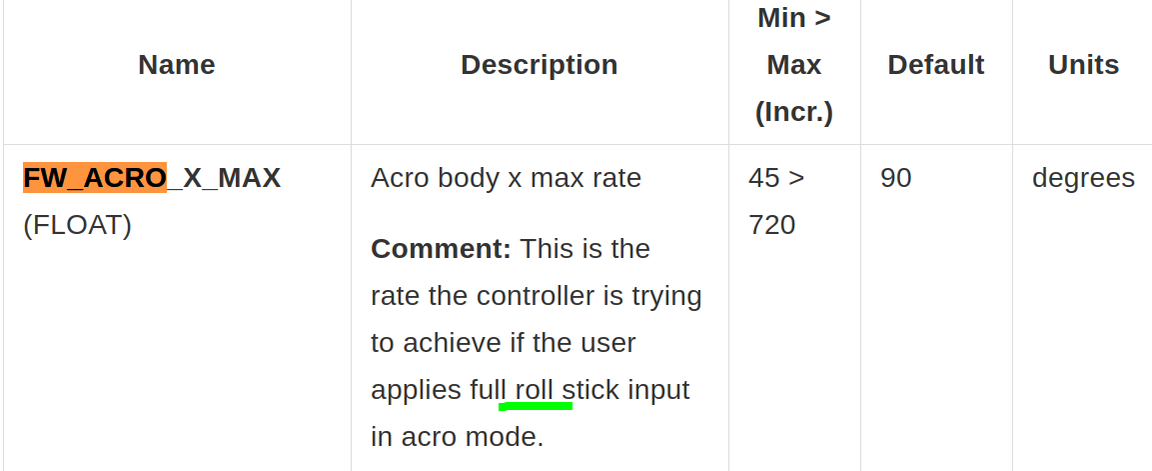
\includegraphics[width=0.48\textwidth]{pictures/parameter1.png}
  }
  \subfigure[y and z]{
      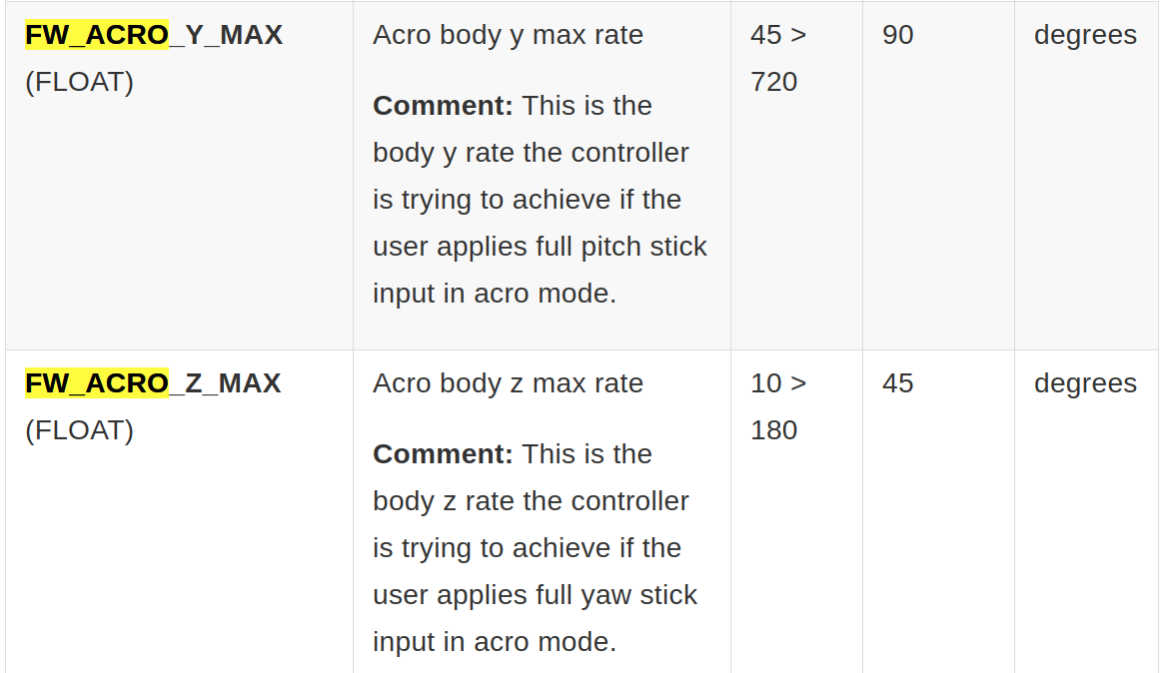
\includegraphics[width=0.48\textwidth]{pictures/att_parameter2.png}
  }
  \caption{parameters}
  \label{fig:param}
\end{figure}
其中各个参数的描述见\ref{fig:param}, 在px4中分别对应的值为\ref{equ:config}. 实现了各个参数的初始化之后, 进行下面的处理
\begin{equation}
  \begin{split}
  roll_{bodyrateSetpoint} &= [\dot{roll} - sin(pitch_{current}) * \dot{yaw}]\\
                          &.constrained[-FW\_ACRO\_X\_MAX, FW\_ACRO\_X\_MAX] \\    
  pitch_{bodyrateSetpoint} &= [cos(roll_{current})*\dot{roll} + cos(pitch_{current}) * sin(roll_{current}) * \dot{yaw}]\\
                          &.constrained[-FW\_ACRO\_Y\_MAX, FW\_ACRO\_Y\_MAX]\\
  yaw_{bodyrateSetpoint} &= [-sin(roll_{current}) * \dot{pitch} + cos(roll_{current}) * cos(pitch_{current}) * \dot{yaw}] \\
                          &.constrained[-FW\_ACRO\_Z\_MAX, FW\_ACRO\_Z\_MAX]
  \end{split}
\end{equation}
最终将上面约束过的体变化率当做姿态的设定值, 发布给下面的控制器以及执行器
\begin{equation}
  \begin{split}
    roll_{setpoint} &= roll_{bodyrateSetpoint} \\
    pitch_{setpoint} &= pitch_{bodyrateSetpoint} \\
    yaw_{setpoint} &= yaw_{bodyrateSetpoint}  
  \end{split}
\end{equation}
\subsection{欧拉角, 四元数的相互转换}
\subsubsection{欧拉角转换为四元数}

\begin{lstlisting}[title=欧拉角转换为四元数]
  void euler_2_quaternion(float angle[3], float quat[4])
  {
      // q0 q1 q2 q3
      // w x y z
      double cosPhi_2 = cos(double(angle[0]) / 2.0);
      double sinPhi_2 = sin(double(angle[0]) / 2.0);
      double cosTheta_2 = cos(double(angle[1]) / 2.0);
      double sinTheta_2 = sin(double(angle[1]) / 2.0);
      double cosPsi_2 = cos(double(angle[2]) / 2.0);
      double sinPsi_2 = sin(double(angle[2]) / 2.0);
      
      quat[0] = float(cosPhi_2 * cosTheta_2 * cosPsi_2 + sinPhi_2 * sinTheta_2 * sinPsi_2);
      quat[1] = float(sinPhi_2 * cosTheta_2 * cosPsi_2 - cosPhi_2 * sinTheta_2 * sinPsi_2);
      quat[2] = float(cosPhi_2 * sinTheta_2 * cosPsi_2 + sinPhi_2 * cosTheta_2 * sinPsi_2);
      quat[3] = float(cosPhi_2 * cosTheta_2 * sinPsi_2 - sinPhi_2 * sinTheta_2 * cosPsi_2);
  }  
\end{lstlisting}

\subsubsection{四元数转换为欧拉角}
\begin{lstlisting}[title=四元数转换为欧拉角]
  Quaternion(const Euler<Type> &euler)
    {
        Quaternion &q = *this;
    
        Type cosPhi_2 = Type(cos(euler.phi() / Type(2)));
        Type cosTheta_2 = Type(cos(euler.theta() / Type(2)));
        Type cosPsi_2 = Type(cos(euler.psi() / Type(2)));
        Type sinPhi_2 = Type(sin(euler.phi() / Type(2)));
        Type sinTheta_2 = Type(sin(euler.theta() / Type(2)));
        Type sinPsi_2 = Type(sin(euler.psi() / Type(2)));
        q(0) = cosPhi_2 * cosTheta_2 * cosPsi_2 +
               sinPhi_2 * sinTheta_2 * sinPsi_2;
        q(1) = sinPhi_2 * cosTheta_2 * cosPsi_2 -
               cosPhi_2 * sinTheta_2 * sinPsi_2;
        q(2) = cosPhi_2 * sinTheta_2 * cosPsi_2 +
               sinPhi_2 * cosTheta_2 * sinPsi_2;
        q(3) = cosPhi_2 * cosTheta_2 * sinPsi_2 -
               sinPhi_2 * sinTheta_2 * cosPsi_2;
}
\end{lstlisting}

\subsection{针对offboard对px4的更改}
在 \textcolor{red}{$fw\_att\_control.cpp$} 控制器中, 对yaw重新计算的时候, 使用的是 $roll_{setpoint}$ 而不是根据当前的roll进行两次约束之后得到的结果. 同时
也去掉$cos(pitch_{current})$这一项.

\section{RC control}
\subsection{raspberry's handled logic and px4's receiver}
树莓派的控制指令以mavlink消息$(MAVLINK_MSG_ID_RC_CHANNELS_OVERRIDE = 70)$进入到px4内部, 处理函数名字为:
\begin{lstlisting}[title=mavlink处理函数声明体]
    // Firmware/src/modules/mavlink/mavlink_receiver.cpp
    void MavlinkReceiver::handle_message(mavlink_message_t *msg);
\end{lstlisting}
\par 处理函数内部会对信息进行解码处理,得到18个通道(channels)的值,并且赋值给 $input\_rc\_s$ rc{}变量, 之后进行
有效性的处理(判断值18个通道的值是否为65535或者是0, 若是, 则该通道的值变为0; 反之, 该通道的值不变,且更新$rc.channel\_count$的值),
处理之后, 使用发布器 $\_rc\_pub$ 将该变量发布到 \\ $ORB\_ID(input\_rc)$话题上(定义发布器的时候, 会设置到PublicationMulti机制, 实例化会有一个优先级的赋值, 可以参见\textcolor{red}{需要补充} )
树莓派发送的四个值占用前四个通道,这个四个通道对应的顺序和遥控器对应指令的通道是不一样的 $(roll = 1 , pitch = 2, throttle = 3, yaw = 4)$.
\begin{lstlisting}[title=$input\_rc\_s$结构体的定义]
    struct input_rc_s {
        uint64_t timestamp;
        uint64_t timestamp_last_signal;
        uint32_t channel_count;
        int32_t rssi;
        uint16_t rc_lost_frame_count;
        uint16_t rc_total_frame_count;
        uint16_t rc_ppm_frame_length;
        uint16_t values[18];
        bool rc_failsafe;
        bool rc_lost;
        uint8_t input_source;
        uint8_t _padding0[3]; // required for logger
    }
    // publisher declaration 
    uORB::PublicationMulti<input_rc_s>			_rc_pub{ORB_ID(input_rc), ORB_PRIO_LOW};
\end{lstlisting}
\begin{lstlisting}[title=树莓派以及固件通道定义]
    // raspberry
    #define PITCH_CHANNEL 		1
    #define ROLL_CHANNEL 		2
    #define YAW_CHANNEL 		3
    #define THROTTLE_CHANNEL 	4
    
    // px4
    #define PITCH_CHANNEL 		1
    #define ROLL_CHANNEL 		2
    #define YAW_CHANNEL 		3
    #define THROTTLE_CHANNEL 	4
\end{lstlisting}

\subsection{其他部分的订阅}

mavlink接收函数拿到数据之后,进行一些处理之后, 将数据publish出去。在$rc\_update$中进行订阅
(multi publish 及其 subscribe 机制在后续文章中进行讲解),订阅器定义如下:
\begin{lstlisting}[title=订阅器的声明定义]
    // src/modules/sensors/rc_update.h
    uORB::Subscription	_rc_sub{ORB_ID(input_rc)};				/**< raw rc channels data subscription */
\end{lstlisting}

在源文件中$rc\_poll\ api$中进行更新获取该变量的值,再进行一些逻辑标志位的检索,
最后对其进行第二次的有效性检测(将每个通道的值约束到某一个固定的区间, 类似constrained()函数; trim操作, 
准备数据为manual id publish做准备), 再一次更新元素的值. 更新后的值处理.
\begin{itemize}
    \item [(1)] 发布到 ORB\_ID(rc\_channels) 话题上面.
    \item [(2)] 将 struct manual\_control\_setpoint\_s manual = {} 数据进行约束到[-1.0f, 1.0f]之间更新到该变量中,继而 发布到 ORB\_ID(manual\_control\_setpoint) 消息上.
    \item [(3)] 将第二次发布得到的 manual 变量, 赋值给 actuator\_group\_3.control 数组, 发布到\\ ORB\_ID(actuator\_controls\_3)消息上.
\end{itemize}

我们真正关心的消息topic应该是$(1\>, 2\>)$, 也就是 $ORB\_ID(rc\_channels)$ 和 $ORB\_ID(manual\_control\_setpoint)$, 
其中 $ORB\_ID(rc\_channels)$ 会被作用到PWM(遥控器和接收机的通信方式)上,所以,我们只需要关心的就是\\ $ORB\_ID(manual\_control\_setpoint)$ 消息topic即可.
\par
上述变量及其函数定义如下:
\begin{lstlisting}[title=上述变量及其函数定义]
    void RCUpdate::rc_poll(const ParameterHandles &parameter_handles);


    rc_channels_s _rc {};			/**< r/c channel data */
    orb_publish_auto(ORB_ID(rc_channels), &_rc_pub, &_rc, &instance, ORB_PRIO_DEFAULT);
    
    
    struct manual_control_setpoint_s manual = {};
    orb_publish_auto(ORB_ID(manual_control_setpoint), &_manual_control_pub, &manual, &instance,
                ORB_PRIO_HIGH);
    
    
    /* copy from mapped manual control to control group 3 */
    struct actuator_controls_s actuator_group_3 = {};
    /* publish actuator_controls_3 topic */
    orb_publish_auto(ORB_ID(actuator_controls_3), &_actuator_group_3_pub, &actuator_group_3, &instance,
                 ORB_PRIO_DEFAULT);
\end{lstlisting}

\subsection{ORB\_ID(manual\_control\_setpoint)}
这个uORB消息, 在px4内部会被 FixedWing Position Controller , FixedWing Attitude Controller 及其他原件进行订阅使用, 
这里我们需要关心的 FixedWing Position Controller , FixedWing Attitude Controller中的使用情况.
\subsubsection{FixedWing Position Controller}
在制导控制器中, px4会根据当前的throttle期望值, 调用 内部的 TECS, 进行新的姿态设定值, 计算期望空速, pitch, 以及使用其他的逻辑来进行计算 yaw, 以及roll的设定值, 赋值给变量$\_att\_sp$, 从而在最后发布给下一层的姿态控制器. 
\begin{lstlisting}[title=计算一些姿态的设定值]
_att_sp.roll_body = _manual.y * _parameters.man_roll_max_rad;
_att_sp.yaw_body = 0;

const float deadBand = 0.06f;
float factor = 1.0f - deadBand;
float pitch = -(_manual.x + deadBand) / factor;

// calculate the demanded airspeed.
float
FixedwingPositionControl::get_demanded_airspeed()
{
	float altctrl_airspeed = 0; // the demanded airspeed.

	// neutral throttle corresponds to trim airspeed
	if (_manual.z < 0.5f) {
		// lower half of throttle is min to trim airspeed
		altctrl_airspeed = _parameters.airspeed_min +
				   (_parameters.airspeed_trim - _parameters.airspeed_min) *
				   _manual.z * 2;

	} else {
		// upper half of throttle is trim to max airspeed
		altctrl_airspeed = _parameters.airspeed_trim +
				   (_parameters.airspeed_max - _parameters.airspeed_trim) *
				   (_manual.z * 2 - 1);
	}

	return altctrl_airspeed;
}
\end{lstlisting}

\textcolor{red}{上述代码公式转换如下}

\subsubsection{FixedWing Attitude Controller}
姿态控制器拿到数据且赋值给 $\_manual$ 变量.
\begin{lstlisting}[title=高度处理逻辑]
if (_vcontrol_mode.flag_control_rattitude_enabled) {
	if (fabsf(_manual.y) > _parameters.rattitude_thres || fabsf(_manual.x) > _parameters.rattitude_thres) {
		_vcontrol_mode.flag_control_attitude_enabled = false;
	}
}
\end{lstlisting}
\par
\begin{itemize}
    \item 若该变量的y和x大于 $\_parameters.rattitude\_thres$ 参数的值, 则 $flag\_control\_attitude\_enabled = false$, 若这个时候$flag\_control\_rates\_enabled$ 为真, 那么执行处理逻辑1; 再将值发布到\\$ORB\_ID(vehicle\_rates\_setpoint)$消息上, 进行下一步的处理.
    \item 若该变量的y和x小于等于 $\_parameters.rattitude\_thres$ 参数的值, 则 $flag\_control\_attitude\_enabled = true$, 执行处理逻辑2, 将值publish到 $\_attitude\_setpoint\_id$ 上面(这个topic就对应offboard从mavros发送到px4的控制逻辑层)
    \item 若不符合上面两个逻辑, 直接执行处理逻辑3, 将控制指令直接发布给执行器. 将值publish到 \\ $\_attitude\_setpoint\_id$ 上
\end{itemize}
\begin{lstlisting}[title=处理逻辑1]  
    _rates_sp.roll = _manual.y * _parameters.acro_max_x_rate_rad;
    _rates_sp.pitch = -_manual.x * _parameters.acro_max_y_rate_rad;
    _rates_sp.yaw = _manual.r * _parameters.acro_max_z_rate_rad;
    _rates_sp.thrust_body[0] = _manual.z;        
\end{lstlisting}
\begin{lstlisting}[title=处理逻辑2]  
    // STABILIZED mode generate the attitude setpoint from manual user inputs
					_att_sp.timestamp = hrt_absolute_time();

					// calculate the setpoints 
					_att_sp.roll_body = _manual.y * _parameters.man_roll_max + _parameters.rollsp_offset_rad;
					_att_sp.roll_body = math::constrain(_att_sp.roll_body, -_parameters.man_roll_max, _parameters.man_roll_max);
					_att_sp.pitch_body = -_manual.x * _parameters.man_pitch_max + _parameters.pitchsp_offset_rad;
					_att_sp.pitch_body = math::constrain(_att_sp.pitch_body, -_parameters.man_pitch_max, _parameters.man_pitch_max);
					_att_sp.yaw_body = 0.0f;
					_att_sp.thrust_body[0] = _manual.z;

					// get the Quatf
					Quatf q(Eulerf(_att_sp.roll_body, _att_sp.pitch_body, _att_sp.yaw_body));
					q.copyTo(_att_sp.q_d);
                    _att_sp.q_d_valid = true;  
                    
                    _attitude_setpoint_id = ORB_ID(vehicle_attitude_setpoint);
\end{lstlisting}
\begin{lstlisting}[title=处理逻辑3]  	
    /* manual/direct control */
    _actuators.control[actuator_controls_s::INDEX_ROLL] = _manual.y * _parameters.man_roll_scale + _parameters.trim_roll;
    _actuators.control[actuator_controls_s::INDEX_PITCH] = -_manual.x * _parameters.man_pitch_scale + _parameters.trim_pitch;
    _actuators.control[actuator_controls_s::INDEX_YAW] = _manual.r * _parameters.man_yaw_scale + _parameters.trim_yaw;
    _actuators.control[actuator_controls_s::INDEX_THROTTLE] = _manual.z;

    _actuators_id = ORB_ID(actuator_controls_0);
\end{lstlisting}

\begin{lstlisting}[title=$\_attitude\_setpoint\_id$]
_attitude_setpoint_id = ORB_ID(vehicle_attitude_setpoint);
\end{lstlisting}

\subsection{Low pass filter}
\begin{lstlisting}[title=Low pass filter from px4]
    float LowPassFilter2p::apply(float sample)
{
	// do the filtering
	float delay_element_0 = sample - _delay_element_1 * _a1 - _delay_element_2 * _a2;

	if (!PX4_ISFINITE(delay_element_0)) {
		// don't allow bad values to propagate via the filter
		delay_element_0 = sample;
	}

	const float output = delay_element_0 * _b0 + _delay_element_1 * _b1 + _delay_element_2 * _b2;

	_delay_element_2 = _delay_element_1;
	_delay_element_1 = delay_element_0;

	// return the value. Should be no need to check limits
	return output;
}
\end{lstlisting}
    
\subsection{数据流}
总体设计阶段以比较抽象概括的方式提出了解决问题的办法。详细设计阶段的任务就是把解法具体化,也就是回答下面这个关键问题:“应该怎样具体地实现这个系统呢?”
这个阶段的任务还不是编写程序,而是设计出程序的详细规格说明。这种规格说明的作用很类似于其他工程领域中工程师经常使用的工程蓝图,它们应该包含必要的细节,程序员可以根据它们写出实际的程序代码。
通常用HIPO图(层次图加输入/处理/输出图)或PDL语言(过程设计语言)描述详细设计的结果。

        \clearpage
    \section{编码和单元测试}
      本项目代码采用面向对象高级编程语言C++编写而成. 采用CMake编译构建系统. 